% Copyright 2025  Ed Bueler

\documentclass[10pt,hyperref,colorlinks]{beamer}

\mode<presentation>
{
  \usetheme{Madrid}

  \usecolortheme{beaver}

  \setbeamercovered{transparent}
  
  \setbeamerfont{frametitle}{size=\large}
}

\setbeamercolor*{block title}{bg=red!10}
\setbeamercolor*{block body}{bg=red!5}

\usepackage[english]{babel}
\usepackage[latin1]{inputenc}
\usepackage{times}
\usepackage[T1]{fontenc}
% Or whatever. Note that the encoding and the font should match. If T1
% does not look nice, try deleting the line with the fontenc.

\usepackage{empheq}
\usepackage{animate}
\usepackage{bm,xspace,verbatim,fancyvrb}
\usepackage{minted}

\usepackage{hyperref}

% If you wish to uncover everything in a step-wise fashion, uncomment
% the following command: 
%\beamerdefaultoverlayspecification{<+->}

\newcommand{\bb}{\mathbf{b}}
\newcommand{\bc}{\mathbf{c}}
\newcommand{\bbf}{\mathbf{f}}
\newcommand{\bg}{\mathbf{g}}
\newcommand{\br}{\mathbf{r}}
\newcommand{\bx}{\mathbf{x}}
\newcommand{\by}{\mathbf{y}}
\newcommand{\bv}{\mathbf{v}}
\newcommand{\bu}{\mathbf{u}}
\newcommand{\bw}{\mathbf{w}}

\newcommand{\bzero}{\bm{0}}

\newcommand{\hbn}{\hat{\mathbf{n}}}

\newcommand{\grad}{\nabla}
\newcommand{\Grad}{\grad}
\newcommand{\Div}{\nabla\cdot}
\newcommand{\Curl}{\nabla\times}

\newcommand{\CC}{\mathbb{C}}
\newcommand{\RR}{\mathbb{R}}

\newcommand{\ddt}[1]{\ensuremath{\frac{\partial #1}{\partial t}}}
\newcommand{\ddx}[1]{\ensuremath{\frac{\partial #1}{\partial x}}}
\newcommand{\Matlab}{\textsc{Matlab}\xspace}
\newcommand{\Octave}{\textsc{Octave}\xspace}
\newcommand{\eps}{\epsilon}

\renewcommand{\Re}{\text{Re}}
\newcommand{\buold}{\bu^{\text{old}}}
\newcommand{\dx}{\,dx}
\newcommand{\dS}{\,dS}

\newcommand{\mfile}[1]{
\VerbatimInput[frame=single,label=\fbox{\scriptsize \textsl{\,#1\,}},fontfamily=courier,fontsize=\scriptsize]{#1}
}

\DefineVerbatimEnvironment{mVerb}{Verbatim}{numbersep=2mm,framerule=0.1mm,framesep=2mm,xleftmargin=4mm,fontsize=\small}


\AtBeginSection[]
{
  \begin{frame}<beamer>
    \frametitle{Outline}
    \tableofcontents[currentsection,hideallsubsections]
  \end{frame}
}

\title{Navier-Stokes solved with finite elements}

\subtitle{in Firedrake}

\author{Ed Bueler}

\institute{MATH 692 Fluids \& Solids Seminar}

\date{Spring 2025}


\begin{document}
\beamertemplatenavigationsymbolsempty

\begin{frame}
  \maketitle
\end{frame}


\begin{frame}{assumptions}

\begin{itemize}
\item all examples here are for 2D domains $\Omega \subset \RR^2$
\item notation: \, $\bu(t,x,y)$ is velocity and $p(t,x,y)$ is pressure
\item density $\rho>0$ is constant
    \begin{itemize}
    \item[$\circ$] fluid is incompressible
    \end{itemize}
\item dynamic viscosity $\mu>0$ is constant
    \begin{itemize}
    \item[$\circ$] constitutive relation: \, $\sigma = -p I + 2 \mu D\bu$
    \end{itemize}
\item body force set to zero: \, $\bbf = \bzero$

\bigskip
\item units:
\begin{align*}
    [\bu]&=\text{m}\,\text{s}^{-1} \\
    [p]&=\text{N}\,\text{m}^{-2} \\
    [\rho]&=\text{kg}\,\text{m}^{-3} \\
    [\mu]&=\text{kg}\,\text{m}^{-1}\,\text{s}^{-1}
\end{align*}
\end{itemize}
\end{frame}


\begin{frame}{the Navier-Stokes model}

\begin{itemize}
\item the time-dependent, incompressible, constant-viscosity Navier-Stokes equations are:
\begin{align*}
\rho\left(\bu_t + \bu \cdot \grad \bu\right) &= \mu \grad^2 \bu - \grad p & &\text{conservation of momentum} \\
\Div \bu &= 0 & &\text{incompressibility (c.~of mass)}
\end{align*}
\end{itemize}
\end{frame}


\begin{frame}{potential flow past a cylinder}

\begin{itemize}
\item recall from 2 weeks ago that Nick provided formula for the potential flow past a cylinder
\item in a \alert{potential flow} the vorticity is zero: \, $\bm{\omega}=\Curl\bu=\bzero$
\item incompressible potential flows satisfy:
\begin{align*}
\Curl \bu &= 0 & &\text{conservation of momentum} \\
\Div \bu &= 0 & &\text{incompressibility (c.~of mass)}
\end{align*}
\item zero curl ($\Curl\bu=0$) so there exists a potential $\bu = \grad \phi$
\item \dots and by incompressibility $\phi$ is harmonic: \, $\grad^2 \phi = 0$
\item assume far field velocity $\bu=(U_0,0)$
\item assume non-penetration and free slip on circle $r=a$
\item get by separation of variables:
	$$\phi(r,\theta) = U_0 \left(r + \frac{a^2}{r}\right) \cos(\theta) \hspace{2.3in}$$
\end{itemize}
\end{frame}


\begin{frame}{potential flow past a cylinder}

\begin{itemize}
\item potential:
	$$\phi(r,\theta) = U_0 \left(r + \frac{a^2}{r}\right) \cos\theta \hspace{2.3in}$$
\item velocity $\bu = \grad \phi$:
{\scriptsize
    $$\hspace{-4mm} \bu(r,\theta) = U_0 \left(1 - \frac{a^2}{r^2}\right) \cos\theta \,\hat \br - U_0 \left(1 + \frac{a^2}{r^2}\right) \sin\theta \,\hat \theta \hspace{3in}$$
}
\item \emph{however}, the boundary condition

along the cylinder, non-penetration

and free slip, is not realistic for

a viscous fluid
\item in fact there is substantial

vorticity along the cylinder
\item and flow separation \dots
\end{itemize}

\vspace{-50mm}
\hfill 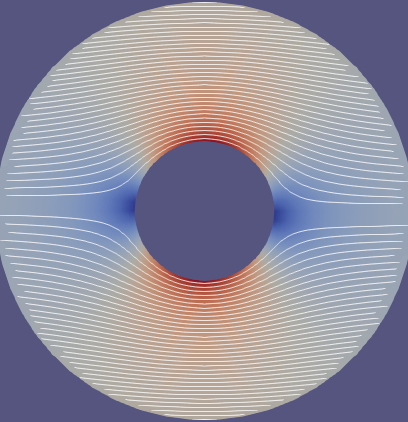
\includegraphics[width=0.45\textwidth]{figs/flowcyl.png}
\end{frame}


\begin{frame}{plan for today}

\begin{itemize}
\item use Firedrake to solve Navier-Stokes (NS) in two situations:
    \begin{enumerate}
    \item lid-driven cavity on a square \hfill \alert{$\leftarrow$ \emph{DEMO NOW!}}
    \item flow around a cylinder on a custom mesh
    \end{enumerate}

\medskip
\begin{center}
\mbox{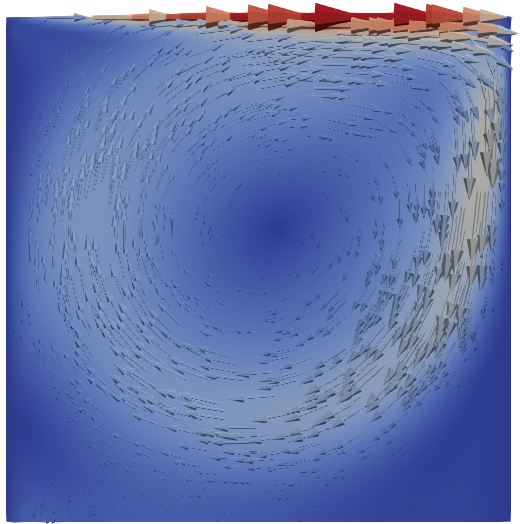
\includegraphics[height=0.33\textheight]{figs/teaser-cavity.png} \hspace{5mm} 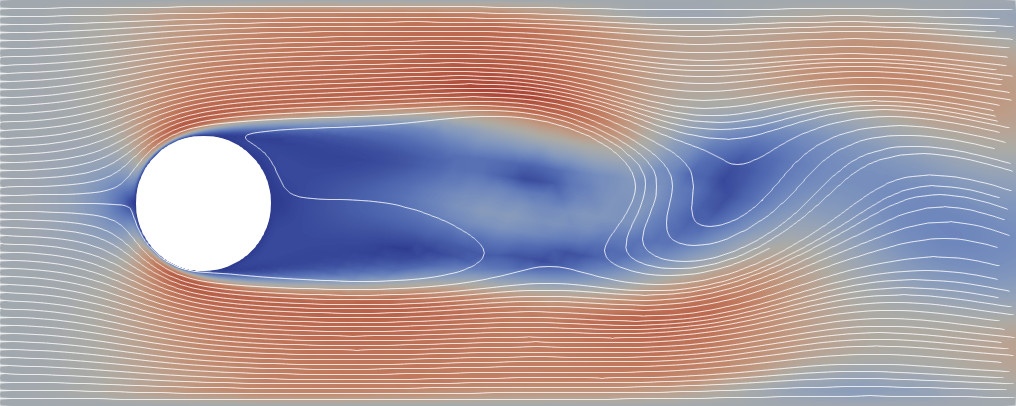
\includegraphics[height=0.32\textheight]{figs/teaser-cylinder.png}}
\end{center}

\medskip
\item TO DO today:
    \begin{itemize}
    \item[$\circ$] the Reynolds scaling argument, to reduce \# of parameters
    \item[$\circ$] implicit discretization of Navier-Stokes (in time)
    \item[$\circ$] weak form
    \item[$\circ$] practical Firedrake coding
    \item[$\circ$] visualization with Paraview
    \item[$\circ$] meshing with Gmsh
    \end{itemize}
\end{itemize}
\end{frame}


\begin{frame}{Reynolds number}

\begin{itemize}
\item recall NS equations:
\begin{align*}
\rho\left(\bu_t + \bu \cdot \grad \bu\right) &= \mu \grad^2 \bu - \grad p, \qquad 
\Div \bu = 0
\end{align*}
\item a particular simulation sets several scales:
    \begin{itemize}
    \item[] $\rho$ density
    \item[] $\mu$ dynamic viscosity
    \item[] $L$ (how long and wide is the domain?)
    \item[] $V$ (how fast is the fluid, e.g.~at boundaries?)
    \end{itemize}
\item one can change variables in the NS model using these substitutions:
    $$\bu = V \tilde \bu, \qquad p = \rho V^2 \tilde p, \qquad \grad = \frac{1}{L} \tilde \grad, \qquad \frac{\partial}{\partial t} = \frac{V}{L} \frac{\partial}{\partial \tilde t}$$

    \begin{itemize}
    \item[$\circ$] the new variables have tildes: \, $\bu,p,x,t \to \tilde \bu,\tilde p,\tilde x,\tilde t$
    \item[$\circ$] the new variables are dimensionless
    \end{itemize}
\end{itemize}
\end{frame}


\begin{frame}{Reynolds number}

\begin{itemize}
\item one rewrites the NS equations using the tilde variables \dots
\item drop the tildes:
\begin{align*}
\bu_t + \bu \cdot \grad \bu &= \frac{\mu}{\rho V L} \grad^2 \bu - \grad p, \qquad 
\Div \bu = 0
\end{align*}
\item note that the coefficient is dimensionless:
	$$\frac{[\mu]}{[\rho] [V] [L]} = \frac{(\text{kg}\,\text{m}^{-1}\,\text{s}^{-1})}{(\text{kg}\,\text{m}^{-3}) (\text{m}\,\text{s}^{-1}) (\text{m})} = 1$$
\end{itemize}
\begin{definition} the \emph{Reynold's number} is the dimensionless ratio
	$$\Re = \frac{\rho V L}{\mu}$$
\end{definition}
\end{frame}


\begin{frame}{Reynolds number}

\begin{itemize}
\item dimensionless NS equations used from now on ($\Re = \rho V L/\mu > 0$):
\begin{align*}
\bu_t + \bu \cdot \grad \bu &= \frac{1}{\Re} \grad^2 \bu - \grad p \\
\Div \bu &= 0
\end{align*}
\item if $\Re$ is small then viscosity is dominant
\item if $\Re$ is large then inertia is dominant
\end{itemize}
\end{frame}


\begin{frame}{implicit time steps}

\begin{itemize}
\item discretization in time typically uses finite differences
\item \emph{key idea}: there is no time derivative in the incompressiblity equation!
    \begin{itemize}
    \item[$\circ$] thus NS equations are really a ``differential-algebraic'' system in time, and infinitely stiff, thus implicitness is a good idea
    \end{itemize}
\item I will use $O(\Delta t)$ backward (implicit) Euler method, highly stable:
	$$\bu_t \approx \frac{\bu^{n} - \bu^{n-1}}{\Delta t}$$
\item suppose $\bu^{n-1}$ is known from previous time step, or initial condition
\item unknowns are $\bu^n$ and $p^n$:
\begin{align*}
\frac{\bu^{n} - \bu^{n-1}}{\Delta t} + \bu^n \cdot \grad \bu^n &= \frac{1}{\Re}\grad^2 \bu^n - \grad p^n \\
\Div \bu^n &= 0
\end{align*}

    \begin{itemize}
    \item[$\circ$] these equations are continuous in space
    \end{itemize}
\end{itemize}
\end{frame}


\begin{frame}{implicit time steps}

\begin{itemize}
\item cleaner notation $\bu=\bu^n$, $p=p^n$, $\buold = \bu^{n-1}$
\item also clear $\Delta t$ from denominator \dots get:

\begin{block}{implicit-step Navier-Stokes equations}
\begin{align*}
\bu - \buold + \Delta t \left(\bu \cdot \grad \bu - \frac{1}{\Re}\grad^2 \bu + \grad p\right) &= 0 \\
\Div \bu &= 0
\end{align*}
\end{block}

\item we will solve these equations for $\bu,p$ \alert{at every time step}, over the domain $\Omega$, using the boundary conditions, and using $\buold$ from the previous time step or the initial conditions
\end{itemize}
\end{frame}


\begin{frame}{weak form of NS equations}

\begin{itemize}
\item above equations are the ``strong form'', in which $\bu$ must have second derivatives and $p$ must have first derivatives
\item this is not necessary, and in finite element (FE) method not desirable
\item the \alert{weak form} is built by multiplying by test functions and integrating
\item multiply 1st equation by $\bv$ and 2nd $q$, and integrate:
{\small
\begin{align*}
\int_\Omega (\bu - \buold)\cdot \bv \dx + \Delta t \int_\Omega \left(\bu \cdot \grad \bu - \frac{1}{\Re}\grad^2 \bu + \grad p\right) \cdot \bv \dx &= 0 \\
\int_\Omega (\Div \bu) q \dx &= 0
\end{align*}
}
\item integrate by parts to remove 2nd deriv from $\bu$ and 1st deriv from $p$:
{\scriptsize
\begin{align*}
\int_\Omega \left(- \tfrac{1}{\Re}\grad^2 \bu + \grad p\right) \cdot \bv \dx &= \int_\Omega \Div \left[- \tfrac{1}{\Re}(\grad \bu)\bv + p \bv\right] \dx - \int_\Omega - \tfrac{1}{\Re} \grad \bu : \grad\bv + p (\Div\bv) \dx \\
&= \int_\Omega \tfrac{1}{\Re} \grad \bu : \grad\bv - p (\Div\bv) \dx + \underbrace{\int_{\partial \Omega} \left(p I - \tfrac{1}{\Re}\grad \bu\right) \hbn \cdot \bv \dS}_{\text{boundary integral}}
\end{align*}
}
\end{itemize}
\end{frame}


\begin{frame}{boundary conditions}

\begin{itemize}
\item two boundary conditions considered here, on separate parts of boundary
\item \alert{stress free} (Neumann):
   $$\left(p I - \tfrac{1}{\Re}\grad \bu\right) \hbn=\bzero$$

    \begin{itemize}
    \item[$\circ$] test functions $\bv$ unrestricted on this part of boundary
    \end{itemize}
\item \alert{given velocity} (Dirichlet):
   $$\bv \, \text{ given}$$

    \begin{itemize}
    \item[$\circ$] test functions satisfy $\bv=\bzero$ on this part of boundary
    \end{itemize}

\medskip
\item assuming one or the other applies everywhere on boundary, then the boundary integral on last slide is zero
\end{itemize}
\end{frame}


\begin{frame}{weak form}

\begin{block}{implicit-step Navier-Stokes equations in weak form}
\begin{align*}
\int_\Omega (\bu - \buold)\cdot \bv \dx + \Delta t \int_\Omega \left(\frac{1}{\Re}\grad \bu : \grad \bv + (\bu \cdot \grad \bu)\cdot \bv - p \Div \bv\right) \dx &= 0 \\
\int_\Omega (\Div \bu) q \dx &= 0
\end{align*}
for all test velocities $\bv$, with $\bv=0$ on Dirichlet boundary, and for all test pressures $q$
\end{block}

\begin{itemize}
\item the problem is nonlinear in $\bu$
\item but the weak form is linear in $\bv$ and $q$
\item note: no derivatives on $p,q$, and only first derivatives on $\bu,\bv$
\end{itemize}
\end{frame}


\begin{frame}[fragile]{weak form in Firedrake}

\begin{align*}
\int_\Omega (\bu - \buold)\cdot \bv \dx + \Delta t \int_\Omega \left(\frac{1}{\Re}\grad \bu : \grad \bv + (\bu \cdot \grad \bu)\cdot \bv - p \Div \bv\right) \dx &= 0 \\
\int_\Omega (\Div \bu) q \dx &= 0
\end{align*}

\medskip
becomes

\medskip
\begin{minted}{python}
F = dot(u - uold, v) * dx
    + dt * (1.0 / Re) * inner(grad(u), grad(v)) * dx
    + dt * dot(grad(u) * u, v) * dx
    - dt * p * div(v) * dx
    - div(u) * q * dx
\end{minted}
\end{frame}


\begin{frame}[fragile]{solver in Firedrake: lid-driven cavity}

\begin{minted}[fontsize=\footnotesize]{python}
mesh = UnitSquareMesh(32, 32)            # Firedrake utility mesh

V = VectorFunctionSpace(mesh, "CG", 2)   # P2 x P1 finite elements
W = FunctionSpace(mesh, "CG", 1)
Z = V * W
up = Function(Z)

u, p = split(up)
v, q = TestFunctions(Z)
F = ...                                  # previous slide

x, y = SpatialCoordinate(mesh)
bcs = [DirichletBC(Z.sub(0), as_vector([4 * x * (1-x), 0.0]), (4,)),
       DirichletBC(Z.sub(0), Constant((0.0, 0.0)), (1, 2)),]

t = 0.0
uold.interpolate(as_vector([0.0, 0.0]))  # initial velocity zero
u, p = up.subfunctions
spar = { ... }                           # for Newton solver
for j in range(N):
    solve(F == 0, up, bcs=bcs, solver_parameters=spar)
    t += dt
    uold.interpolate(u)
\end{minted}
\end{frame}


\begin{frame}{demonstrations}

\begin{itemize}
\item Python codes are in \texttt{py/bueler/} directory of repository

\begin{center}
 \href{https://github.com/bueler/fluid-solid-seminar}{\texttt{github.com/bueler/fluid-solid-seminar}}
\end{center}
\item you will need to get \href{https://www.firedrakeproject.org/}{Firedrake} installed to use these
\end{itemize}

\bigskip
\begin{enumerate}
\item demo: lid-driven cavity on a square
    \begin{itemize}
    \item[$\circ$] look at \href{https://github.com/bueler/fluid-solid-seminar/blob/main/py/bueler/navierstokes.py}{\texttt{navierstokes.py}} and \href{https://github.com/bueler/fluid-solid-seminar/blob/main/py/bueler/cavity.py}{\texttt{cavity.py}}
    \item[$\circ$] visualize with \href{https://www.paraview.org/}{Paraview}
    \end{itemize}

\bigskip
\item demo: flow around a cylinder on a custom mesh
    \begin{itemize}
    \item[$\circ$] build mesh using \href{http://gmsh.info/}{Gmsh}, using geometry-description file \href{https://github.com/bueler/fluid-solid-seminar/blob/main/py/bueler/cylinder.geo}{\texttt{cylinder.geo}}
    \item[$\circ$] look at \href{https://github.com/bueler/fluid-solid-seminar/blob/main/py/bueler/navierstokes.py}{\texttt{navierstokes.py}} and \href{https://github.com/bueler/fluid-solid-seminar/blob/main/py/bueler/cylinder.py}{\texttt{cylinder.py}}
    \item[$\circ$] visualize with \href{https://www.paraview.org/}{Paraview}
    \item[$\circ$] play with Reynold's number
    \end{itemize}
\end{enumerate}
\end{frame}




\end{document}

